\documentclass{beamer}

\definecolor{kugreen}{RGB}{46,83,84}
\definecolor{kugreenlys}{RGB}{86,157,160}
\definecolor{kugreenlyslys}{RGB}{165,165,165}
\definecolor{kugreenlyslyslys}{RGB}{242,242,242}
\definecolor{kugreenclaro}{RGB}{192, 213, 184}
\definecolor{ocre}{RGB}{244, 236, 187}
\definecolor{ocreclaro}{RGB}{251, 249, 217}
\mode<presentation>
{
  \usetheme{Rochester}      % or try Darmstadt, Madrid, Warsaw, ...
  \usecolortheme[named=kugreen]{structure} % or try albatross, beaver, crane, ...
  \usefonttheme{structureitalicserif}  % or try serif, structurebold, ...
\setbeamertemplate{navigation symbols}{}
  \setbeamertemplate{caption}[numbered]
} 

\usepackage[english]{babel}
\usepackage[utf8x]{inputenc}

\usepackage[]{graphicx}
\usepackage[]{color}
\usepackage{geometry}
\usepackage{multimedia}



\newtheorem{defi}{Definici\'on}[section]
\newtheorem{ej}{Ejemplo}[section]
\newtheorem{ejs}{Ejemplos}[section]
\newtheorem{prop}{Proposici\'on}[section]
\newtheorem{nota}{Nota}[section]
\newtheorem{notac}{Notación}[section]
\newtheorem{rem}{Observaci\'on}[section]
\newtheorem{thm}{Teorema}[section]
\newtheorem{cor}{Corolario}[section]
\newtheorem{lem}{Lema}[section]
\newtheorem*{dem}{Demostración}

\title[El problema paramétrico del emparejamiento en grafos y problema de emparejamiento con dos objetivos]{\textbf{\textup{El problema paramétrico del emparejamiento en grafos y problema de emparejamiento con dos objetivos}}}
\author{Rafael González López\\ Supervisado por: Justo Puerto Albondoz\\}
\institute{Universidad de Sevilla}
\date{\textit{Departamento de Estadística e investigación Operativa}}

\begin{document}

%%%%%%%%%%%%%%%%%%%%%%%%%%%%%%%%%%%%%%%%%%%%%%%%%%%%%%%%%%%%%%%%%%%%%

\begin{frame}
  \titlepage
\end{frame}

%%%%%%%%%%%%%%%%%%%%%%%%%%%%%%%%%%%%%%%%%%%%%%%%%%%%%%%%%%%%%%%%%%%%%%

\begin{frame}{Índice}
 \tableofcontents
\end{frame}

%%%%%%%%%%%%%%%%%%%%%%%%%%%%%%%%%%%%%%%%%%%%%%%%%%%%%%%%%%%%%%%%%%%%%%


\section{Introducción}
\subsection{Problema de emparejamiento}

\begin{frame}{¿Qué es un emparejamiento en un grafo?}
\begin{figure}[h!]
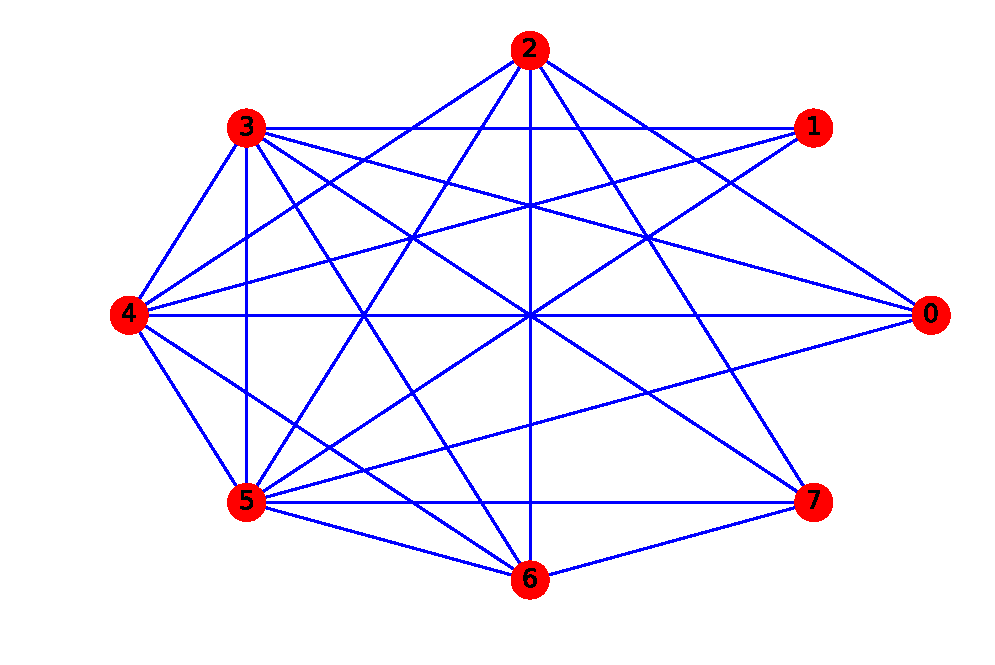
\includegraphics[scale=0.45]{opt}
\end{figure}
\end{frame}

%%%%%%%%%%%%%%%%%%%%%%%%%%%%%%%%%%%%%%%%%%%%%%%%%%%%%%%%%%%%%%%%%%%%%%
\subsection{Formulación del problema}
\begin{frame}{Formulación del problema}
\begin{figure}[h!]
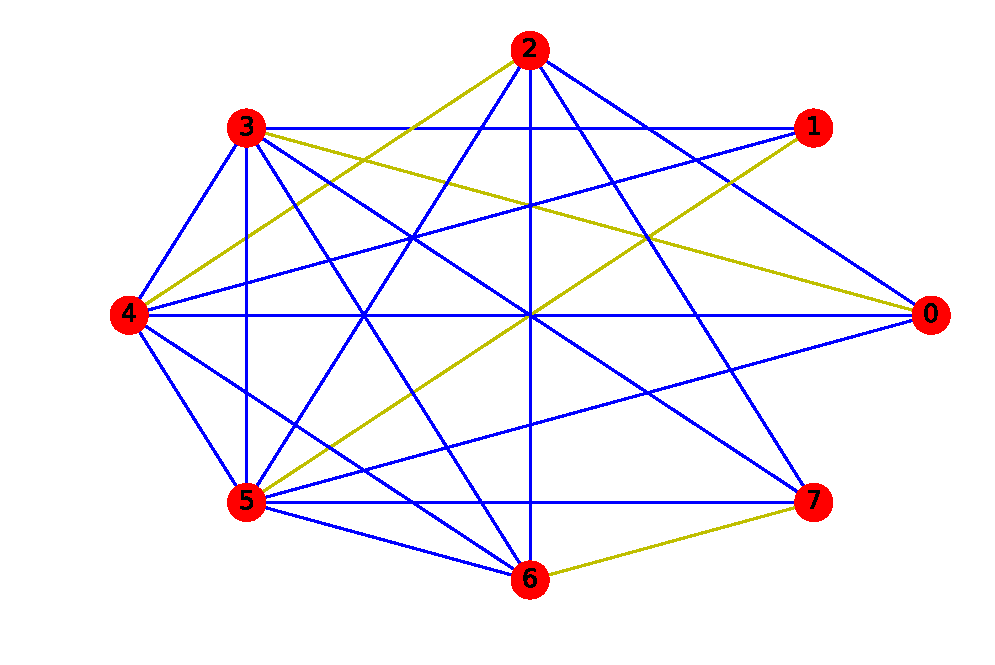
\includegraphics[scale=0.45]{opt2}
\end{figure}
\end{frame}

\begin{frame}{Problema de optimización}
Sea $G=(V,E)$ un grafo. Entonces podemos considerar:
\begin{align*}
\max_{x} &\; \sum_{(u,v)\in E} x_{uv}c_{uv}  \nonumber\\ 
s.a.\;  &  Ax\leq b \\
& x\in\{0,1\}^n\nonumber
\end{align*}
donde $c$ es el vector de pesos, $A$ es la matriz de incidencia del grafo, $|E|=n$ y la variable $x_{uv}=1$ si la arista $(u,v)$ está en el emparejamiento y $0$ en caso contrario.
\end{frame}

\begin{frame}{Definiciones previas}
\begin{defi}
Sea $G=(V,E)$ y $W\subset V$. Entonces 
\begin{gather*}
\delta(W) = \{(u,v)\in E \mid \text{Exactamente $u \in W$ o $w \in W$} \}\\
\gamma(W) = \{(u,v)\in E \mid u,v \in W\}
\end{gather*}
\end{defi}
\end{frame}
\begin{frame}{Teorema de Edmonds}
\begin{thm}
Sea $G=(V,E)$ un grafo. Sea $B$ el conjunto
$$
B = \{S\subset V \mid |S| \text{ es impar},\;|S|\geq 3\}
$$
Entonces, la envolvente convexa del politopo del matching viene dada por
\begin{align*}
\sum_{(u,v)\in\delta(u)} x_{uv} &\leq 1, \quad \forall u\in V\\
x_{uv} &\geq 0\\
\sum_{(u,v)\in \gamma(S)} x_{uv}& \leq \frac{1}{2}(|S|-1)\quad \forall S \in B	
\end{align*}
\end{thm}
\end{frame}

\subsection{Problemas estudiados}
\begin{frame}{Emparejamiento perfecto de mínimo peso}
\begin{align*}
\min_x & \sum_{(u,v) \in E}x_{uv}c_{uv}\\
s.a.&\;\sum_{(u,v)\in\delta(u)} x_{uv} = 1, \quad \forall u \in V\\
&\sum_{(u,v)\in \gamma(S)} x_{uv} \leq \frac{1}{2}(|S|-1)\quad \forall S \in B	\\
&x_{uv} \geq 0 \qquad \forall(u,v)\in E
\end{align*}
\end{frame}
\begin{frame}{Problema paramétrico}\begin{align*}
\min_x & \sum_{(u,v) \in E}x_{uv} (c_{uv} + \lambda d_{uv})\\
s.a.&\;\sum_{(u,v)\in\delta(u)} x_{uv} \leq 1, \quad \forall u \in V\\
&\sum_{(u,v)\in \gamma(S)} x_{uv} \leq \frac{1}{2}(|S|-1)\quad \forall S \in B	\\
&x_{uv} \geq 0 \qquad \forall(u,v)\in E
\end{align*}
donde $d_{uv} = I_R((u,v))$.
\end{frame}
\begin{frame}{Problema biobjetivo}
\begin{align*}
\min_x & \left(\sum_{(u,v) \in E}x_{uv}c^1_{uv},\sum_{(u,v) \in E}x_{uv} c^2_{uv}\right)\\
s.a.&\;\sum_{(u,v)\in\delta(u)} x_{uv} \leq 1, \quad \forall u \in V\\
&\sum_{(u,v)\in \gamma(S)} x_{uv} \leq \frac{1}{2}(|S|-1)\quad \forall S \in B	\\
&x_{uv} \geq 0 \qquad \forall(u,v)\in E
\end{align*}
\end{frame}
\subsection{Grötschel-Holland}
\begin{frame}{Problemas de la formulación de Edmonds}
\begin{itemize}
\item La formulación de Edmonds tiene un número exponencial de restricciones en el número de vértices.
\item Para grafos incluso medianos resulta infactible computacionalmente.
\item Grötschel y Holland proponen un algoritmo para lidiar con este problema y utilizar Programación Lineal.
\end{itemize}
\end{frame}

\begin{frame}{Algoritmo de Grötschel-Holland}
\begin{enumerate}
\item Determinamos $NN$ y $E'\subset E$.
\item Resolvemos el problema
\begin{align*}
\min_x & \sum_{(u,v) \in E'}x_{uv}c_{uv}\\
s.a.&\;\sum_{(u,v)\in\delta(u)} x_{uv} = 1, \quad \forall u \in V\\
&x_{uv} \geq 0 \qquad \forall(u,v)\in E'
\end{align*}
\end{enumerate}

\end{frame}
\end{document}